\chapter{Approach}
% Describe the performed solution with all possible details. Define necessary parameters, inputs, outputs and context of use, possible problems and when they can be applied. 

% Remember to define necessary concepts before using them, building the text from easiest definitions (not depending on previous definitions) to complex definitions (depending on previous definitions).

% E.g: 
% \begin{itemize}
%	\item Lost Communication: a lost communication occurs when the conditions of the environment are not sufficient or the distance between sender and receiver is to hight to transmit information.
%	\item Wait until rescue: when the robot loses its communication, the pre-designed state machine will stop the motors to keep the actual position. Energy safe mode will be enabled, at the same time that a channel transceiver daemon will send SOS messages every T and wait for reply during T sec. 
%\end{itemize}
In our system there are multiple robots that must handle various tasks. For example, visiting given rooms. To tackle this problem, a communication efficient task scheduling system is designed. 
This system allocate task according to system resources, including environment factors, robot status and task specifications. Once this information is attained, the task scheduling system assign robot a set of task.

\begin{itemize}
	\item \textsl{Robot.} Each robot is responsible for moving in 2-dimensional physical space as well as gathering measurement result from sensors. It has a rechargeable battery, and its level drops as robot moves and rotates.
	\item \textsl{Tasks.} Each task requires one or more robots to traverse a path in the workspace and carry out certain actions\cite{Ivan2017}.
	\item \textsl{Environment.} In this project, all robots are considered moving in an office environment that contains a corridor along the central x-axis and 16 rooms located around the corridor. The environment factors, such as room locations and occupancy possibilities help task allocation.
\end{itemize}

\section{Architecture Design}

The architecture of the system consist of several parts: centralized pool, robot controller, navigation stack, charging station and system environment(Figure \ref{fig:system_architecture}). 
\begin{itemize}
	\item \textsl{Centralized Pool.} A centralized pool consist of several modules: multi-robot task allocation module, map information, database, execution and monitoring. The database contains most of the environment information(Figure \ref{fig:database_er}). The multi-robot task allocation module allocate tasks to robots once requested.
	\item \textsl{Robot Controller.} A robot controller contains several modules: local task queue, execution and robot action. The execution module receives commands from centralized pool and decides when and which task the robot should perform.
	\item \textsl{Navigation stack.} The move\_base node provides a ROS interface for configuring, running, and interacting with the navigation stack on a robot. It makes robot move to desired positions using the navigation stack. Its advantages include optionally performing recovery behaviors when the robot perceives itself as stuck\cite{move_base_node}. 
\end{itemize} 

\begin{figure}[htbp]
	\centering
	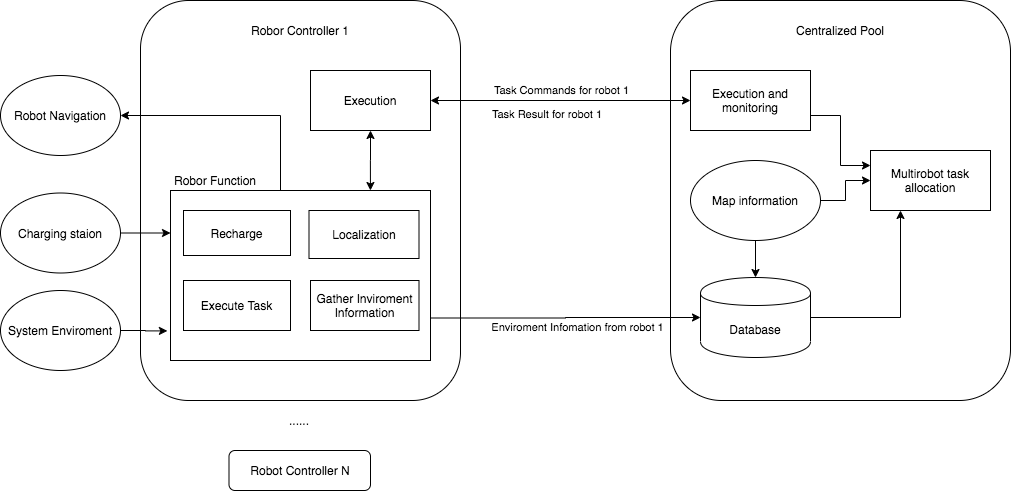
\includegraphics[width = 0.9\textwidth]{content/images/ch3/architecture.drawio.png}
	\caption{System Architecture}
	\label{fig:system_architecture}
\end{figure}

\section{System Environment}
\label{sec:system_enviroment}
As is discussed in the previous section, the system environment is an office environment. The SLAM (Simultaneous Localization and Mapping) is a technique to draw a map by estimating current location in an arbitrary space \cite{slam}. Map (Figure \ref{fig:room_division}) is created by SLAM.


There are following important areas and coordinates:
\begin{itemize}
	\item \textsl{Rooms.} The rectangle areas (Figure \ref{fig:room_division}) are used to represent Rooms. Each rectangle has its upper and lower limit in x and y coordinates. The system uses those limits to determine a position in which room. 
	\item \textsl{Doors.} The positions of doors (Figure \ref{fig:positions_door_station}) are stored in database. There are used by a ROS door simulator node, which broadcasts positions and door status periodically. The broadcast messages are received and filtered by robots.
	\item \textsl{Charging Stations.} The positions of charging stations are used by ROS charging station nodes. For details please refer to Section \ref{sec:charging_station}.
\end{itemize}

\begin{figure}[htbp]
	\centering
	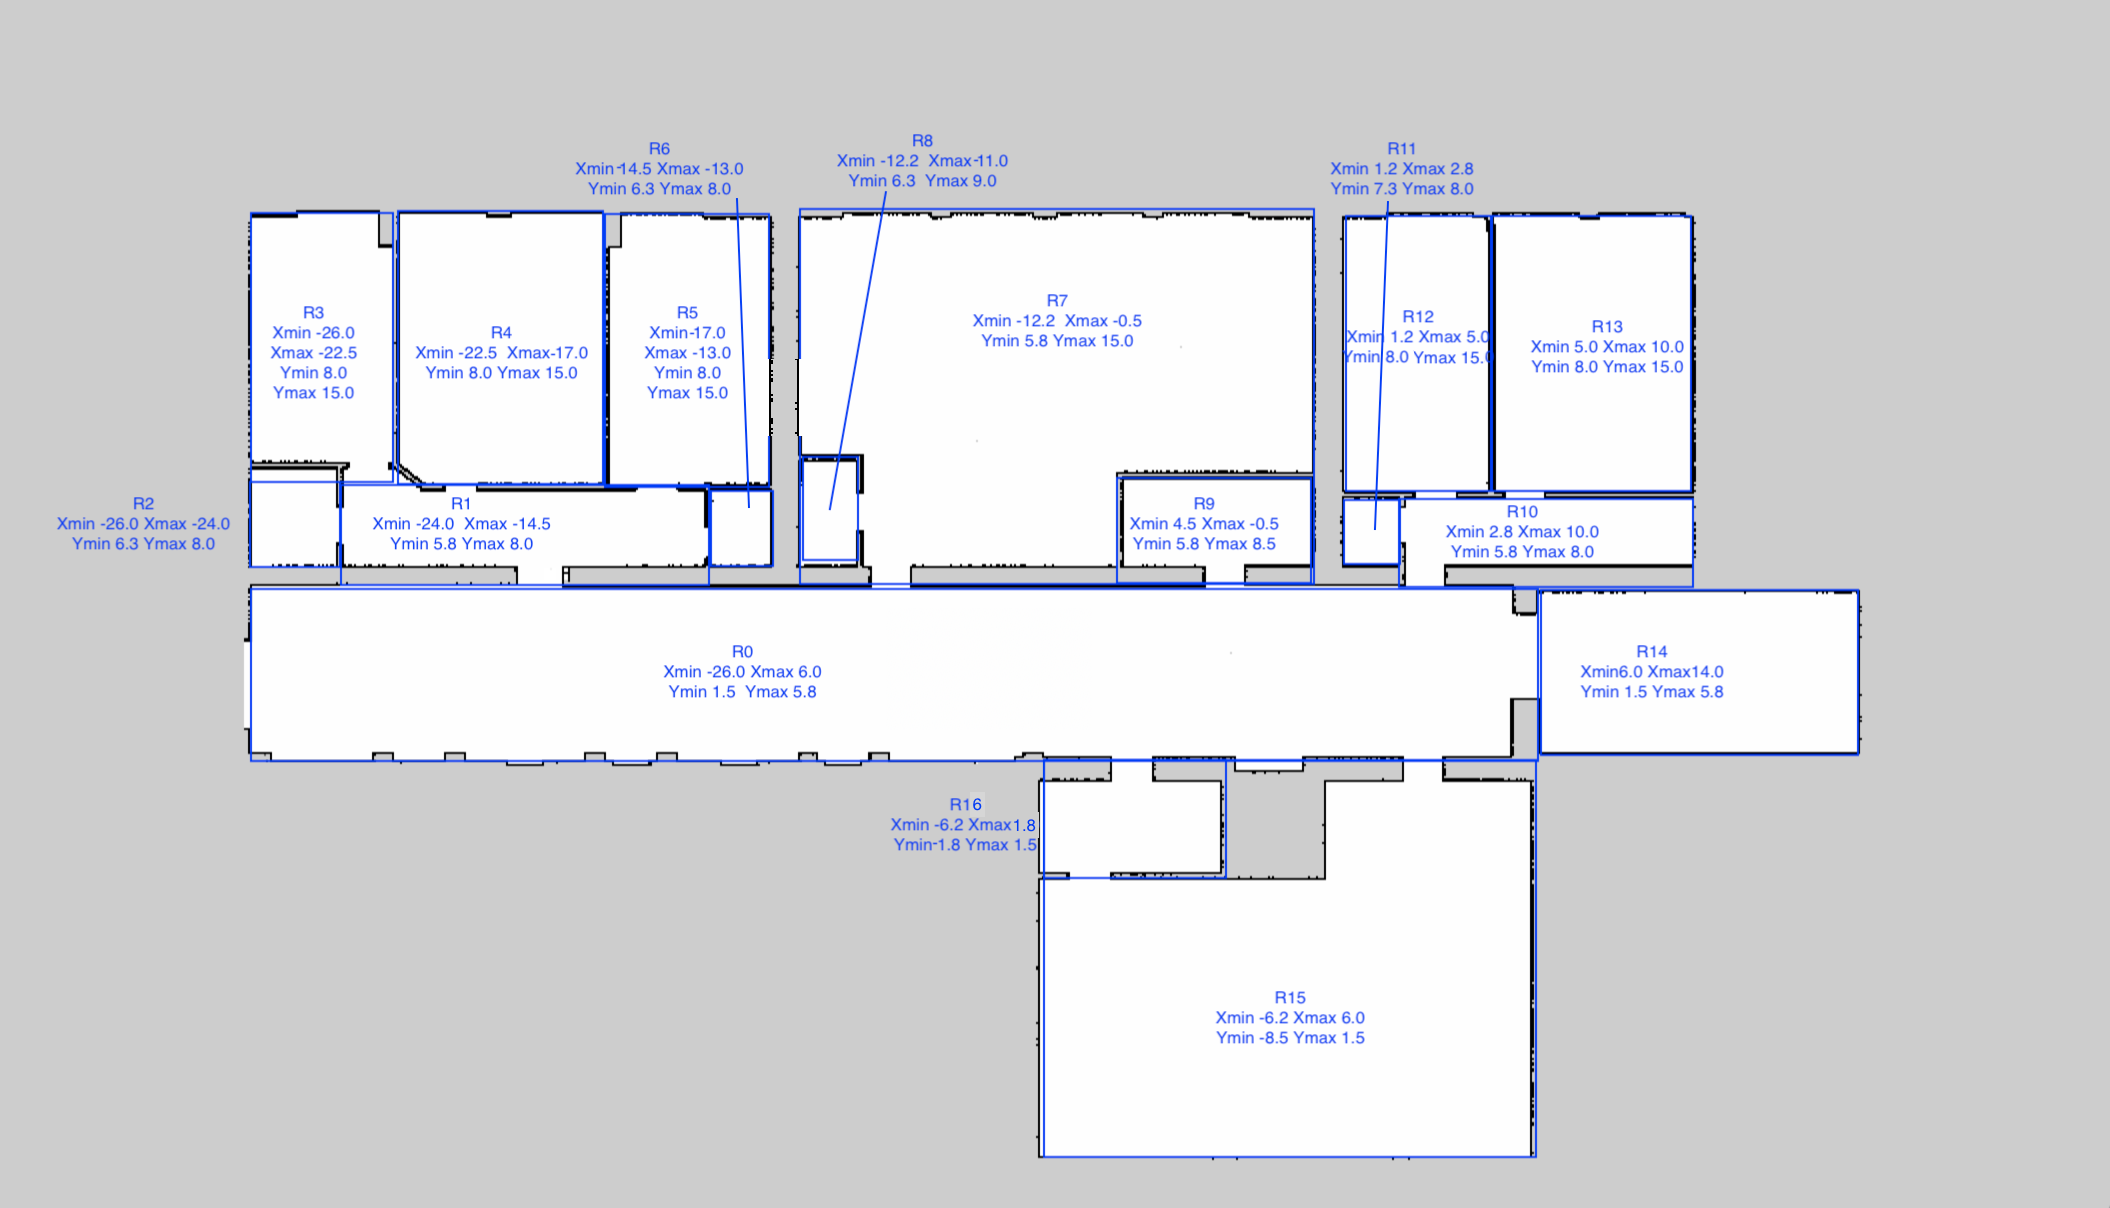
\includegraphics[width = 0.9\textwidth]{content/images/ch3/room_division.png}
	\caption{Room division}
	\label{fig:room_division}
\end{figure}

\begin{figure}[htbp]
	\centering
	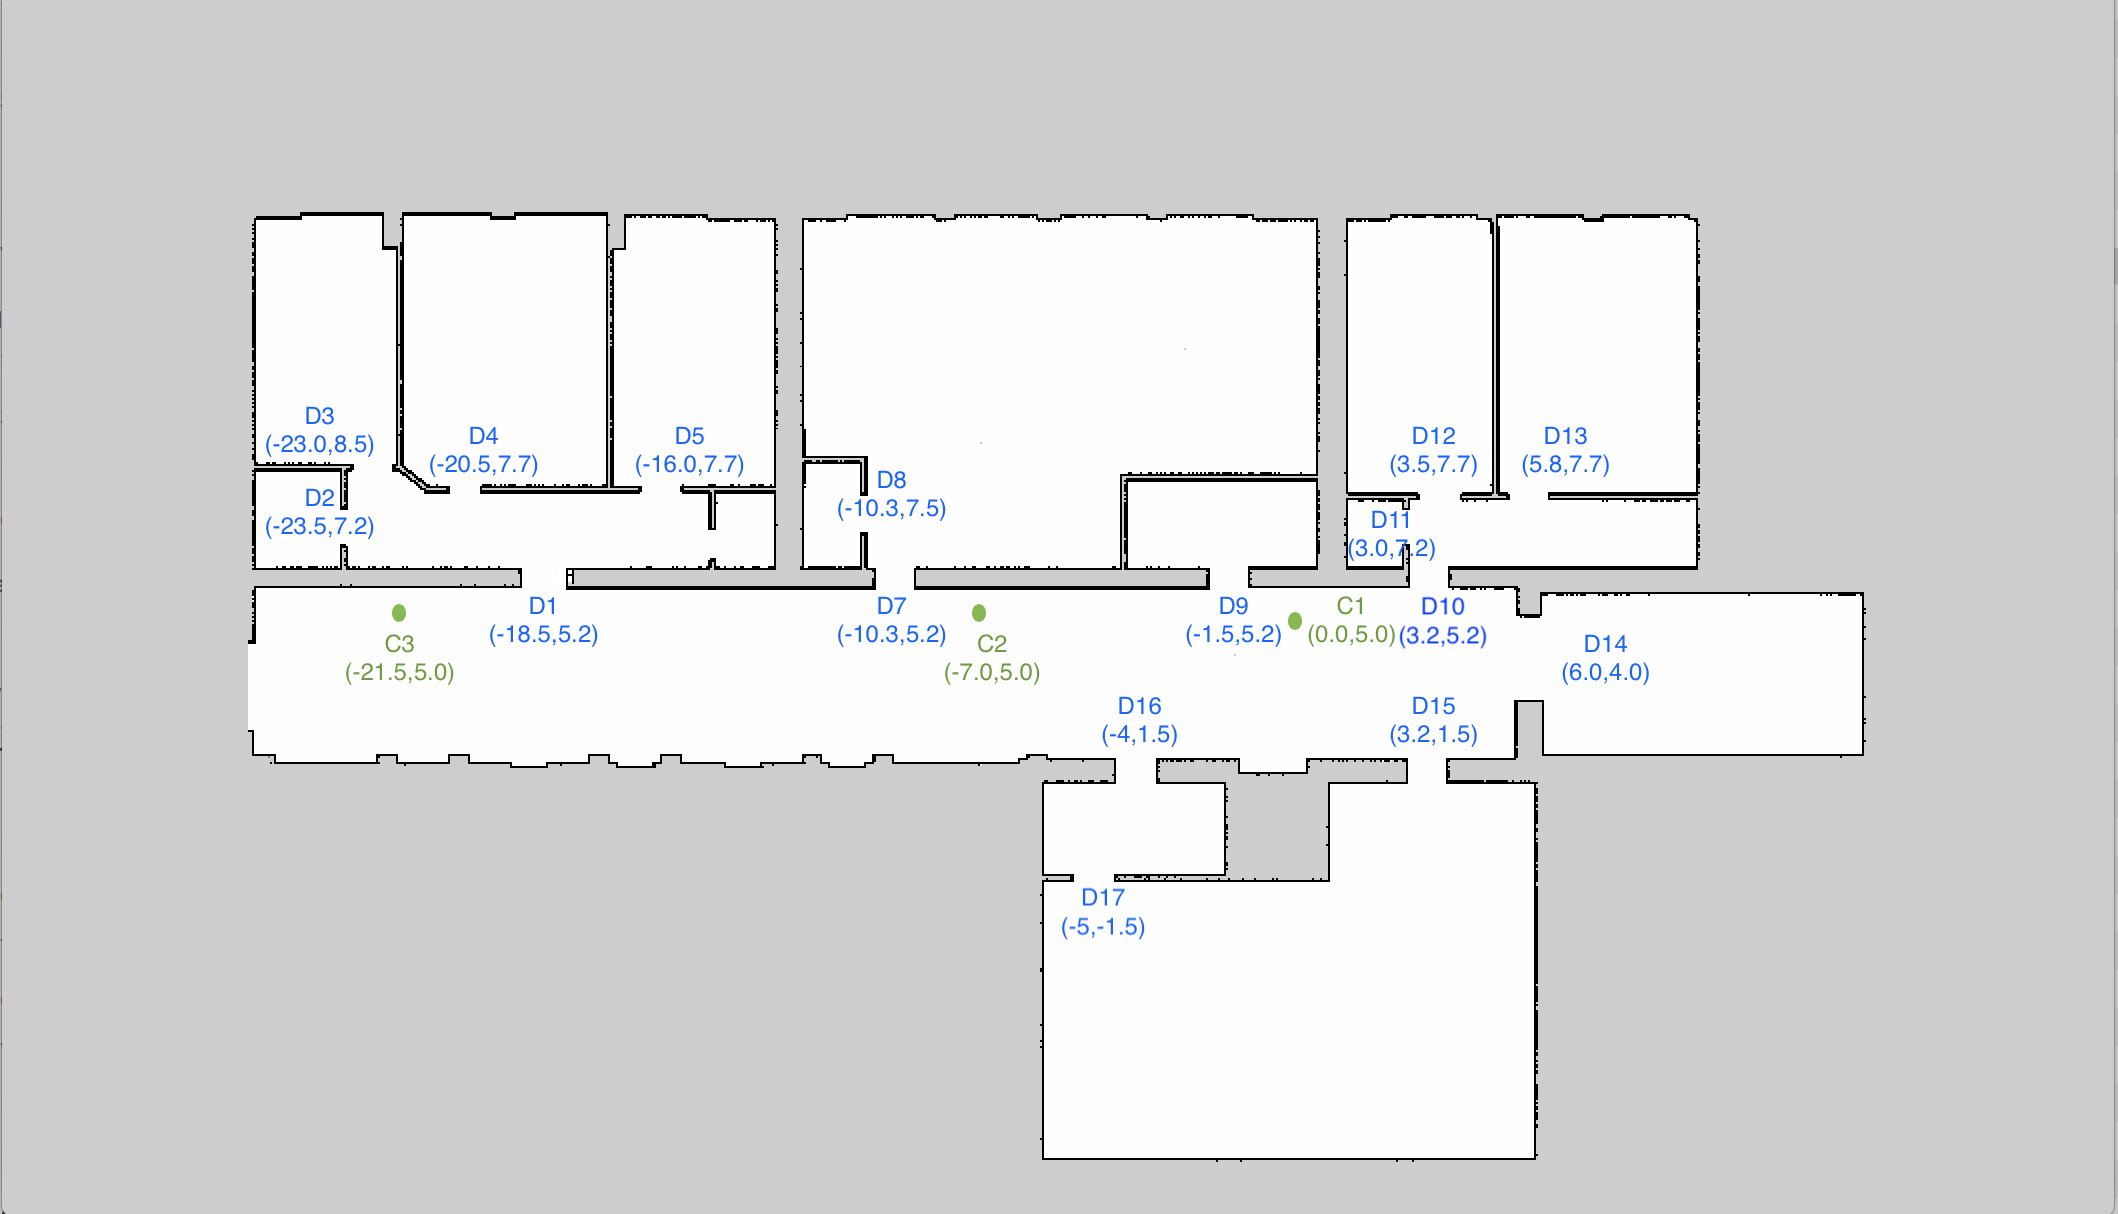
\includegraphics[width = 0.9\textwidth]{content/images/ch3/positions_door_station.png}
	\caption{Doors and Charging Stations}
	\label{fig:positions_door_station}
\end{figure}

\section{Task Allocation}

\subsection{Task Specifications}
\label{sec:task_specifications}
On one hand, recharging is necessary for robots to work long hours. On the other hand, a robot should gather environment information as much as possible, which centralized pool would learn from and make better decision. 
Therefore, three types of task are defined. Table (Table \ref{tab:task_specifications} list task specifications. In addition, each task has a ``start time'' when the robot receives the task and a ``finish time'', which robot the sends result)
A task can be classified into small task and large task. 
One robot can carry either small task, which make robot move to one position, or large task, which consist of multiple small task.
\begin{itemize}
	\item Small Task. A small task contains only one goal. When a robot receives a small task, it moves to the only goal. 
	\item Large Task. A large task contains several small tasks, and each small tasks contains a goal. Those small tasks form a dependency chain. When a robot gets a large task, it moves continuously to those goals. The centralized pool can query ``small execute tasks'' and use them to form a ``large execute tasks''.
\end{itemize}

\begin{table}[htb]
\centering
\resizebox{\textwidth}{!}{
\begin{tabular}{|c|c|c|c|c|c|c|c|c|c|} 
\hline
\diagbox{Task type}{Task Specifications} & Target & Dependency & Priority & Generator & Task Size\\
\hline
Gather environment infomation task & Door &  No & 1 & Centralized pool & Small task\\
\hline
Execute task & Any point & Dependent on ``execute task'' & 2,3,4 & User & Small task (in database) or large task (in centralized pool) \\
\hline
Charging Task & Charging station & No & 5 & Centralized Pool & Small task \\ [1ex] 
\hline
\end{tabular}}
\caption{Task Specifications}
\label{tab:task_specifications}
\end{table}



\begin{table}[htb]
\centering
\resizebox{\textwidth}{!}{
\begin{tabular}{|c|c|c|c|c|c|c|c|c|c|} 
\hline
Task ID & Task Type & Start Time & Target ID & Robot ID & Priority & Status & dependency & Finish Time  & Description \\
\hline
1 &  Charging task & 2020-06-01 9:00:00 & 18 & 1 & 5 & RanToCompletion & 0 & 2020-06-01 9:00:20 & Succeeded \\
\hline
2 &  Execute task & 2020-06-01 9:00:50 & 22 & 2 & 2 &RanToCompletion & 0 & 2020-06-01 9:01:20 & Succeeded \\
\hline
3 &  Gather environment information task & 2020-06-01 9:02:00 & 2 & 2 & 1 & Running & 0 & 2020-06-01 9:02:40 & Succeeded \\ [1ex] 
\hline
\end{tabular}}
\caption{Task Table in Database}
\label{tab:task_table}
\end{table}

\begin{itemize}
	\item \textsl{Target.} Targets include doors, points and charging stations. When a robot run a ``gather environment information task'', it moves to the front of a door and interact with a sensor in the door position without entering the door. 
	When robot run an ``execute task'', the robot moves to a given point ether in corridor or in the room.
	When robot run a ``charging task'', the robot moves to a charging station and interact with this charging station.
\end{itemize}

\subsection{Execute Task Allocation}
\label{sec:exe_task_allocation}
With robot status such as positions and available battery provided by robot, the multi-robot task allocation module in the architecture should perform multi-robot task allocation. 
When the centralized pool receives a task request (Table \ref{tab:request_message}) from robot,  the multi-robot task allocation module in the architecture. The implementation of task allocation is shown in Figure \ref{fig:centralized_task_allocation}. 
\begin{enumerate}
	\item When the battery of robot belows 10\%, the centralized pool will create a charging task to the charging staion with the lowest cost.
	\item When the battery of robot aboves 10\%, the centralized pool will load all ``execute tasks'' in database and combine small tasks with dependencies into large tasks(Section \ref{sec:task_specifications}), finally calculate task costs and select one large task with the lowest cost. 
    \item If there are no suitable tasks, a ``gather environment task'' to the door with the lowest cost is generated. 
    \item The output of the task allocation includes: task ID, goal coodinates, timestamp and selected robot ID. The task is sent to the selected robot, and the robot performs the tasks.

\end{enumerate}


\paragraph*{Decision variables}
To select an ``execute task'', the following decision variables are considered.
\begin{itemize}
\item \textsl{Task Priority.} Task Priority. Task priority is an important factor that describes task emergency level. The ``charging task'' has the highest priority of 5. The ``gather environment information'' task has the lowest priority of 1. 
	The ``execute task'' is determined by users but must be in the range of [2,4]. 
\item \textsl{Product of Door Open Possibility.} Because of the limitation of simulation, the door open possibilities are used to represent room occupancies. A door open possibility is based on the statistic of door measurement results in a specific time period of a working day. 
	The doors on trajectory (doors that the robot may pass through) can be obtained from the map information module.
	An example of ``measurement result'' table is shown in Table \ref{tab:db_measurement_result}, an example of ``open possibility'' table is shown in Table \ref{tab:db_open_possibilities}. 
\item \textsl{Waiting Time. } The waiting time is the difference between the current simulation time and start time of the first task to be executed. $T_{waiting} = T_{first\_task} - T_{now}$
\item \textsl{Battery Consumption.} The Battery Consumption is related to robot trajectory. For a Large ``execute task'' that contains n small task, Equation \ref{eq:battery_consumption} can be used to calculate battery consumption. The centralized pool will send the task with the lowest cost to this robot.

\end{itemize}

Equation \ref{eq:large_execute_task_cost} shows how these decition variables are used to calculate the cost of a large ``execute task''.

\todo{Database Table}
\begin{equation}
\begin{aligned}
\label{eq:battery_consumption}
& \mbox{B:Battery consumption } \\
& \mbox{W: Weight } \\
& \mbox{m: Number of waypoint } \\
& \mbox{n: Number of task} \\
& B_{\mbox{large task}} = \sum_{\mbox{task}_1}^{\mbox{task}_n} B_{\mbox{trajectory}} \\
& = \sum_{t = \mbox{task}_1}^{\mbox{task}_n} \sum_{\mbox{waypoint}_1}^{\mbox{waypoint}_m} [W_{\mbox{position}} \times \mbox{position variation}+W_{\mbox{angle}}  \times \mbox{angle variation}]\\
& = \sum_{t = \mbox{task}_1}^{\mbox{task}_n} \sum_{p = \mbox{waypoint}_1}^{\mbox{waypoint}_m} [ W_{\mbox{position}} \times \sqrt{(x_p-x_{p-1} )^2+(y_p-y_{p-1} )^2} \\
&   + W_{\mbox{angle}} \times 2 \times \arccos(w_p)] 
\end{aligned}
\end{equation}


\begin{equation}
	\label{eq:large_execute_task_cost} 
	\begin{aligned}
	& \mbox{W: Weight } \\
	& \mbox{n: Number of doors} \\
	& \mbox{Cost}_{\mbox{Large execute task}} = \frac{W_{\mbox{battery}} \times \mbox{Battery consumtion}}{n} + W_{\mbox{waiting}} \times \mbox{waiting time} \\
	& + W_{\mbox{possibility}} \times \prod\limits_{i=1}^n \mbox{Door open possibility}  + W_{\mbox{priority}} \times \mbox{Priority}
	\end{aligned}
\end{equation}


\subsection{Environment Task Allocation}
As is discussed in section \ref{sec:exe_task_allocation}, once there are no suitable tasks in centralized pool, the task allocation module should create a``gather environment information task'', in order to gather more measurement result and further more improve the accuracy of ``open possibilities'' table.
To create a ``gather environment information task'', which door should the requesting robot visit must be considered. The following decision factors help task allocation module to select the door.

\paragraph*{Decision variables}
\begin{itemize}
	\item \textsl{Door Last Update Time.} The latest timestamp when the door is measured.
	\item \textsl{Battery Consumption.} Similar to ``execute task`` allocation, the battery consumption is related to the trajectory from robot to the door. Equation \ref{eq:battery_consumption} can be used to calculate battery consumption.
	\item \textsl{Whether door is used.} If another robot is going to this door, the value is 0, otherwise the value is 1.
\end{itemize}

\begin{equation}
	\label{eq:door_cost}
	\begin{aligned}
	& \mbox{W: Weight } \\
	& \mbox{n: Number of doors on trajectory} \\	
	& \mbox{Cost}_{\mbox{door}} = \frac{W_{\mbox{battery}} \times \mbox{Battery consumtion}}{n} + W_{\mbox{time}} \times (T_{\mbox{last update}} - T_{\mbox{now}}) \\
	& + W_{\mbox{possibility}} \times \prod\limits_{i=1}^n \mbox{Door open possibility}
	\end{aligned}
\end{equation}

\subsection{Charging Task Allocation}
As is discussed in section \ref{sec:exe_task_allocation}, once a robot sends task request to the centralized pool, the centralized pool should figure out whether this robot need charging, if yes it should create a ``charging task'' for requesting robot. Since there are multiple charging station in the system environment (Figure \ref{fig:positions_door_station}), the centralized pool selects a charging station for this robot using the following decision variables.
\paragraph*{Decision variables}

\begin{itemize}
	\item \textsl{Remain Time.} It describes how long will a charging station be free. 
	\item \textsl{Battery Consumption.} Similar to ``execute task'' allocation, the battery consumption is related to the trajectory from robot to the charging station. Equation \ref{eq:battery_consumption} can be used to calculate battery consumption.
\end{itemize}
In conclusion, equation \ref{eq:charging_station_cost} can be used to calculate the cost of a charging station. The centralized pool will generate a ``charging task'' for requesting robot to charging station with the lowest cost.

\begin{equation}	
\label{eq:charging_station_cost}
\begin{aligned}
	& \mbox{W: Weight } \\
	& \mbox{Cost}_{\mbox{charging station}} = \frac{W_{\mbox{battery}} \times \mbox{battery consumtion}}{n} + W_{\mbox{time}} \times T_{\mbox{remain}}
\end{aligned}
\end{equation}

